%
% teil1.tex -- Beispiel-File für das Paper
%
% (c) 2020 Prof Dr Andreas Müller, Hochschule Rapperswil
%
%
% teil2.tex -- Beispiel-File für teil2 
%
% (c) 2020 Prof Dr Andreas Müller, Hochschule Rapperswil
%%

\rhead{Kalman-Filter}
\section{Kalman-Filter}
Im letzten Abschnitt haben wir Gleichungen für unser System gefunden.
Als nächstes brauchen wir also ein Werkzeug,
um aus der Messung der Position $s(t)$ den gesammten Zustand $x(t)$ zu schätzen.
Das ist genau das, was Kalman-Filter tun:
Anhand von Messungen den Zustand eines Systems schätzen.

Kalman-Filter wurde 1960 von Rudolf Emil Kalman erfunden und direkt von der NASA für die Apollo Mission benutzt.
Diese Filter kommen mit wenig Rechenleistung aus und waren somit geeignet, die Rakete bei der Navigation zu unterstützen. 
Heutige, typische Anwendungen von Kalman-Filtern sind die Glättung verrauschter Daten und die Schätzung von Parametern.
Dies kommt heutzutage in jedem Satellit, Navigationssystem, Smartphone und Videospiel vor.

Kalman-Filter funktionieren nach folgendem Zwei-Schritt-Verfahren:
Zuerst wird,
ausgehend von der aktuellen Schätzung des Zustands und der Eigendynamik des Systzems,
eine Vorhersage berechnet.
Daraus lässt sich eine erwartete Messung ableiten.
Anschliessend wird diese Vorhersage korrigiert,
wobei die Korrektur abhänging von der Differenz zwischen erwarteter und effektiver Messung ist.

Dabei sind sowohl die Vorhersage als auch die Messung nur Schätzungen und unweigerlich fehlerbehaftet.
Unter der Annahme, dass die Fehler normalverteilt sind,
lassen sich beide Schätzungen zu einer neuen, optimalen Schätzung kombinieren.
Die genaue Herleitung des Kalman-Filters ist relativ aufwendig
und kann unter Anderem in \cite{erdbeben:skript:wrstat} nachgelesen werden.

\subsection{Exkurs Wahrscheinlichkeit} 
\label{erdbeben:Wahrscheindlichkeit} 
Das Kalman-Filter schätzt also den wahrscheinlichsten Wert zwischen zwei Normalverteilungen,
genauer gesagt zwischen einer Messung und einer Vorhersage.
In diesem Abschnitt wollen wir auffrischen, wie dies genau passiert.

Das Folgende wird in \cite{erdbeben:aragher_understanding_2012} beschrieben.
Wir haben eine Vorhersage aus der Systemdynamik und eine Messung des Zustandes.
Diese widersprechen sich im Allgemeinen. 
Jedoch kennen wir auch die Wahrscheinlichkeiten der beiden Aussagen. 

\begin{figure}
 \begin{center}
 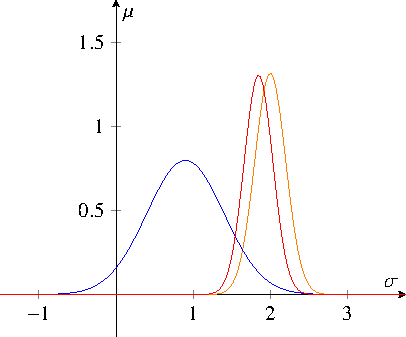
\includegraphics[width=.5\linewidth,keepaspectratio]{papers/erdbeben/Gausskurve3.pdf}
 \caption{
    Seien blau und orange zwei normalverteilte Schätzungen eines Zustandes, etwa eine Vorhersage und eine Messung.
    Dann ist die rote Kurve die optimale Schätzung.
    Sie entspricht bis auf Normierung dem Produkt von blau und orange.}
 \label{erdbeben:Gauss3}
 \end{center}
\end{figure}
Abbildung~\ref{erdbeben:Gauss3} zeigt in blau und rot zwei Normalverteilungen,
je eine für die Vorhersage und eine für die Messung.
Diese unterscheiden sich sowohl in ihren Mittelwerten $\mu_{1,2}$, als auch in ihren Standardabweichungen $\sigma_{1,2}$.
Um eine genauere Schätzung des Zustandes zu machen, wird nun ein Wert zwischen den beiden Verteilungen berechnet. 
Nun wird eine Eigenschaft der Normalverteilung ausgenutzt:
Durch das Multiplizieren zweier Normalverteilungen entsteht eine neue Normalverteilung. 

Wir haben also eine Normalverteilung der Vorhersage
\[ 
{y_1}(x;{\mu_1},{\sigma_1})=\frac{1}{\sqrt{2\pi\sigma_1^2}}\quad e^{-\frac{(x-{\mu_1})^2}{2{\sigma_1}^2}} 
\]
und der Messung
\[ 
{y_2}(x;{\mu_2},{\sigma_2})=\frac{1}{\sqrt{2\pi\sigma_2^2}}\quad e^{-\frac{(x-{\mu_2})^2}{2{\sigma_2}^2}}.
\]
Diesen werden nun multipliziert und durch deren Fläche geteilt,
um sie wieder zu normieren.
$\odot$~beschreibt dabei die Multiplikation und die Normierung auf den Flächeninhalt eins:
\begin{align*}
	{y_f}(x; {\mu_f}, {\sigma_f}) 
	&=
	 {y_1}(x;{ \mu_1},{ \sigma_1}) \odot {y_2}(x; {\mu_2}, {\sigma_2})
	\\
	&=
	\frac{1}{\sqrt{2\pi\sigma_1^2}}\quad e^{-\frac{(x-{\mu_1})^2}{2{\sigma_1}^2}} \odot \frac{1}{\sqrt{2\pi\sigma_2^2}}\quad e^{-\frac{(x-{\mu_2})^2}{2{\sigma_2}^2}}
	\\
	&=
	\frac{ \frac{1}{\sqrt{2\pi\sigma_1^2}}e^{-\frac{(x-{\mu_1})^2}{2{\sigma_1}^2}} \cdot \frac{1}{\sqrt{2\pi\sigma_2^2}}e^{-\frac{(x-{\mu_2})^2}{2{\sigma_2}^2}}}{\int {y_1} {y_2} dx}.
\end{align*}
Die genaue Berechnung ist nicht schwierig aber aufwendig und wird hier deshalb ausgelassen.
Nach einigem Rechnen findet man die Ausdrücke
\[ \mu_f = \frac{\mu_1\sigma_2^2 + \mu_2 \sigma_1^2}{\sigma_1^2 + \sigma_2^2} \]
für den neuen Mittelwert und
\[
\sigma_f^2 = \frac{\sigma_1^2 \sigma_2^2}{\sigma_1^2 + \sigma_2^2}.
\]
für die Varianz.

Interessant daran ist, dass sich die fusionierte Kurve der genaueren Normalverteilung anpasst.
Ist ${\sigma_2}$ klein und ${\sigma_1}$ gross,
so wird sich die fusionierte Kurve näher an ${y_2}(x;{\mu_2},{\sigma_2})$ begeben.
$\mu_f$ ist das gewichtete Mittel der beiden $\mu_{1,2}$, und die Varianzen $\sigma_{1,2}$ sind die Gewichte.
Das Interessante an $\mu_{f}$ ist, dass ${\mu_2}$ das Gewicht für ${\sigma_1}$ ist. 
Somit ist die Unsicherheit der Messung das Gewicht der Vorhersage und umgekehrt.
Diese neue Funktion ist die bestmögliche Schätzung für zwei Verteilungen, welche den selben Zustand beschreiben.
Dies ist in der Abbildung~\ref{erdbeben:Gauss3} anhand der roten Funktion ersichtlich. 

Was in zwei Dimensionen erklärt wurde, funktioniert auch in mehreren Dimensionen. 
Dieses Prinzip mach sich das Kalman Filter zu nutze, und wird von uns für die Erdbebenberechnung genutzt. 

\subsection{Filter-Matrizen}
Da wir nun ein Werkzeug besitzen, dass die Beschleunigung, welche auf das Gehäuse wirkt, ermitteln kann,
wird dies nun Schritt für Schritt erklärt. 
Um das Kalman-Filter zu starten, müssen gewisse Bedingungen definiert werden. 
In diesem Abschnitt werden die einzelnen Parameter und Matrizen erklärt und erläutert, wofür sie nützlich sind. 

Dabei muss genau auf den Index geachtet werden.
Wir verwenden die Standardnotation, wie sie auch im Artikel~\cite{erdbeben:wikipedia} zu finden ist.
Sie ist an die Notation der bedingten Wahrscheinlichkeiten angelehnt.
Hierbei steht der betrachtete Zeitschritt links und der gegenwärtige rechts eines Vertikalstrichs.
Dies bedeutet, dass die Notation $x_{n|m}$ die Schätzung von $x$ zum Zeitpunkt $n$ 
aufgrund des Wissens bis zum und mit dem Zeitpunkt $m$ repräsentiert.

\subsubsection*{Vorhersage}
Im Filterschritt Vorhersage wird anhand des aktuellen Zustands und der Systemmatrix eine Schätzung für den nächsten Zustand berechnet. 
Die Systemmatrix $A$ aus Gleichung~\eqref{erdbeben:systemmatrix} beschreibt ein kontinuierliches System $\dot x = Ax$.
Wir benötigen jedoch ein Zeit-diskretes System $x_{k+1} = \Phi x_k$.

Die Exponentialfunktion $\exp(At)$ beschreibt die Entwicklung eine Zustandes im Laufe der Zeit.
Die Übergangs-Matrix $\Phi$ erhalten wir folglich aus der Systemdynamikmatrix $A$ durch die Exponentialfunktion
\[\Phi = \exp(A\Delta t). \]
Die Matrix $\Phi$ beschreibt die Übergänge zwischen zeitlich aufeinanderfolgenden Zuständen $x_{k-1}$ und $x_{k}$ anhand folgender Gleichung:
\[
{x_{k|k-1}}=\Phi{x_{k-1|k-1}}= \exp(A\Delta t){x_{k-1|k-1}}.
\] 
Damit haben wir die Systemdynamik nun in der für unser Kalman-Filter notwendigen Form und können Vorhersagen berechnen.

Als nächstes benötigen wir die Unsicherheit der Vorhersage.
Im Abschnitt ~\ref{erdbeben:Wahrscheindlichkeit} haben wir dafür die Varianzen der Normalverteilungen verwendet.
Im mehrdimensionalen Fall übernimmt dies die Kovarianzmatrix $P$.
Sie wird in jedem Schritt aktualisiert.
Hinzu kommt die Prozessunsicherheit $Q$, welche als Parameter in unser Modell einfliesst.
$Q$ beschreibt Unsicherheiten im Modell,
wie etwa unsere Annahme, dass die Kraft sich nicht ändert,
aber auch nicht-modellierbare Einflüsse wie Vibrationen.
$P$ wird dabei laufend aktuallisiert.
Die Gleichung lautet
\[
{P_{k|k-1}}=\Phi {P_{k-1|k-1}} {\Phi _{k}}^T + {Q_{k-1}}.
\] 
Es vergeht genau $\Delta t$ Zeit, und dieser Vorgang wird wiederholt.  
Das Filter passt sich selber an und korrigiert sich bei grosser Abweichung.

\subsubsection*{Messen}
Der Sensor wurde noch nicht benutzt, doch genau der liefert die Messwerte $z_k$ für unser Filter. 
Aus der Vorhersage des Zustandes $x_{k|k-1}$ und der Messmatrix $H$ erhalten wird eine Vorhersage der Messung. 
Die Innovation
\[
{w_{k}}={z_{k}}-{H}{x_{k|k-1}}
\] 
beschreibt, wie genau die Vorhersage $x_{k|k-1}$ zur aktuellen Messung $z_k$ passt. 
Die Innovation ist also derjenige Teil der Messung, der nicht im Modell erfasst ist.
Dies leuchtet ein, eine Innovation von $0$ bedeutet, dass die Messung nichts Neues hervorbrachte.
Für eine schlechte Vorhersage wird die dazugehörige Innovation gross, für eine genaue Vorhersage dagegen klein sein. 
Entsprechende Korrekturen werden dann gross bzw. nur gering ausfallen. 

\subsubsection*{Aktualisieren}

Für eine optimale Schätzung des Zustandes muss die Vorhersage entsprechend der Innovation korrigiert werden.
In der Literatur findet man für eine optimales Korrektur die Gleichungen
\begin{align*}
{S_{k}} &={H}{P_{k|k-1}}{H}^T+{R_{k}}
\\
{K_{k}} &= {P_{k|k-1}} {H^T}{S_{k}^{-1}}
\end{align*}
Dabei ist $K$ das Kalman-Gain.
$K$ beschreibt, wie die Vorhersage korrigiert werden muss.
Die optimale Schätzung des neuen Zustandes wird dann zu
\[
{x_{k|k}}={x_{k|k-1}}+{K_{k}}{w_{k}}.
\] 
Dazu kommt eine neue Kovarianz $P$ für den nächste Vorhersageschritt:
\[
{P_{k|k}}=(I-{K_{k}}{H}){P_{k|k-1}}. 
\] 
Der ganze Algorithmus ist nun vollständig und beginnt wieder mit der Vorhersage 
\[
{x_{k+1|k}}=\Phi{x_{k|k}}= \exp(A\Delta t){x_{k|k}}.
\] 


\subsection{Parameter und Anfangsbedingungen}
Die Grössen $P$, $Q$, $R$ und $\Phi$ können grundsätzlich in jedem Zeitschritt ändern.
Für die meisten Anwendungen sind sie jedoch konstant und fliessen als Parameter ins Modell ein.
So auch in unserem Falle.
Aufgrund der iterativen Arbeitsweise von Kalman-Filtern benötigen wir zudem ein paar Anfangswerte.

\subsubsection*{Anfangszustand $x$}
Für die erste Vorhersage benötigt das Filter einen Anfangszustand.
In unserem Fall ist es die Ruhelage, die Masse bewegt sich nicht. 
Zudem erfährt die Apparatur keine äussere Kraft:
\[ {x_0 }= \left( \begin{array}{c} {s_0}\\ {v_0}\\{f_0}\end{array}\right) = \left( \begin{array}{c} 0\\ 0\\ 0\end{array}\right). \]

\subsubsection*{Systemmatrix $A$ und $\Phi$}
Für unseren Seismographen haben wir die entsprechende Matrixdarstellung
in Gleichung~\eqref{erdbeben:systemmatrix} bereits gefunden.
Zudem haben wir weiter oben bereits beschrieben,
wie wir mittels Exponentialfunktion zu einer zeitdiskreten Beschreibung für das Kalman-Filter kommen.
Es gilt
\[ \Phi = \exp(A \Delta t) .\]

\subsubsection*{Anfangsfehler / Kovarianzmatrix $P$}
Da auch der Anfangszustand fehlerhaft sein kann, wird für das Filter eine Anfangsunsicherheit verwendet. 
Auf der Diagonalen werden die Varianzen eingesetzt, in den restlichen Felder stehen die Kovarianzen.
Für einen gut bekannten Zustandsvektor können kleine Werte eingesetzt werden, für ungenaue Anfangsbedingungen sollten grosse Werte verwendet werden. 
Grosse Werte ermöglichen dem Filter sich schnell einzupendeln. 

In unserem Fall ist der Anfangszustand gut bekannt. 
Wir gehen davon aus,
dass das System in Ruhe und in Abwesenheit eines Erdbeben startet.
Somit kann die Matrix mit Nullen bestückt werden und wir starten mit
\[ 
P_0 =
\begin{pmatrix}
0 & 0 &0 \\ 
0 &0 & 0 \\ 
0 & 0 &0 \\
\end{pmatrix}
.
 \] 


\subsubsection*{Prozessrauschkovarianzmatrix $Q$}
Die Prozessrauschmatrix teilt dem Filter mit, wie sich der Prozess verändert. 
Die Matrix $Q$ beschreibt die Unsicherheit, die der Prozess mit sich bringt. 
Bei unserem Modell könnte das beispielsweise ein Windstoss an die Masse sein
oder auch Ungenauigkeiten im Modell, wie die Annahme, dass sich die Kraft nicht ändert.
Für uns wäre dies:
\[ 
Q =
 \begin{pmatrix}
\sigma_s^2& 0& 0 \\ 
0 & \sigma_v ^2& 0\\ 
0 & 0& \sigma_f^2\\
\end{pmatrix} .
 \]
Die Standabweichungen müssten statistisch ermittelt werden, da der Fehler nicht vom Sensor kommt und somit nicht vom Hersteller gegeben ist. 

\subsubsection*{Messmatrix $H$}
Die Messmatrix gibt an, welche Zustände gemessen werden. 
$H$ ist die Matrix, welche aus der Vorhersage des Zustand eine Vorhersage der Messung erzeugt.
In unserem Falle messen wir nur die Position der Massen und verwenden deshalb
\[ 
H = \begin{pmatrix} 1 & 0 & 0 \end{pmatrix} .
\]

\subsubsection*{Messrauschkovarianz $R$}
Die Messrauschkovarianzmatrix beinhaltet, wie der Name schon sagt, das Rauschen der Messung. 
In unserem Fall wird nur die Position der Masse gemessen. Da wir keine anderen Sensoren haben ist $R$ lediglich:
\[ 
R= (\sigma_\mathrm{Sensor}^2).
 \] 
Diese Messrauchen wird meistens vom Sensorhersteller angegeben. 
Für unsere theoretische Apparatur wird hier ein kleiner Fehler eingesetzt,
da heutige Sensoren sehr genau messen können.

\subsection{Zusammenfassung }
Das Filter beginnt mit dem Anfangszustand für $k=0$.
Anschliessend werden folgende Schritte iterativ ausgeführt:
\begin{enumerate}
\item Nächsten Zustand vorhersagen
\[
{x_{k|k-1}}=\Phi{x_{k-1|k-1}}= \exp(A\Delta t){x_{k-1|k-1}}
\] 

 \item Nächste Fehlerkovarianz vorhersagen
\[
{P_{k|k-1}}=\Phi {P_{k-1|k-1}} {\Phi _{k}}^T + {Q_{k-1}}
\] 

\item Innovation (= Messung - Vorhersage)
\[
{w_{k}}={z_{k}}-{H}{x_{k|k-1}}
\] 

\item Optimales Kalman-Gain berechnen
\begin{align*}
{S_{k}} &={H}{P_{k|k-1}}{H}^T+{R_{k}}\\
{K_{k}} &= {P_{k|k-1}} {H^T}{S_{k}^{-1}}
\end{align*}

\item Schätzung aktualisieren
\[
{x_{k|k}}={x_{k|k-1}}+{K_{k}}{w_{k}}
\] 

\item Fehlerkovarianz aktualisieren
\[
{P_{k|k}}=(I-{K_{k}}{H}){P_{k|k-1}}
\] 

\end{enumerate}
Die Outputs von $k$ werden die Inputs für ${k+1}$ und werden wieder in Schritt 1 verwendet.

